\chapter{Marco te\'orico}
\label{cap:marco}

En este capítulo se exponen los conceptos teóricos del presente trabajo de tesis. <Rellenar al final>


\section{Motores de búsqueda verticales}
\label{marco:mbv}
A medida que pasa el tiempo y la Web sigue creciendo, los motores de búsqueda se convierten en una herramienta cada vez más importante para los usuarios. Estas máquinas ayudan a los usuarios a buscar contenido dentro de la Web, puesto que conocen en qué páginas de la Web aparecen qué palabras. Sin un buscador los usuarios estarían obligados a conocer los localizadores de recursos uniformes (URL) de cada uno de los sitios a visitar. Además, los motores de búsquedas en cierto modo conectan la Web, ya que existe un gran número de páginas Web que no tienen referencia desde otras páginas, siendo el único modo de acceder a ellas a través de un motor de búsqueda.

Un motor de búsqueda está construído por diversos componentes, y su arquitectura típica la podemos ver en la Figura \ref{fig:searchenginearchitecture}. Existe un proceso denominado \textit{crawling}, éste posee una tabla con las páginas Web iniciales en las que se extrae el contenido de cada una de ellas. A medida que el \textit{crawler} comienza a encontrar enlaces a otras páginas Web, la tabla de páginas a visitar crece. El contenido que se extrae en el procedimiento de \textit{crawling} es enviado al proceso de indexamiento, este se encarga de crear un índice de las páginas visitadas por el \textit{crawler}. 

\begin{figure}[tp]
\centering
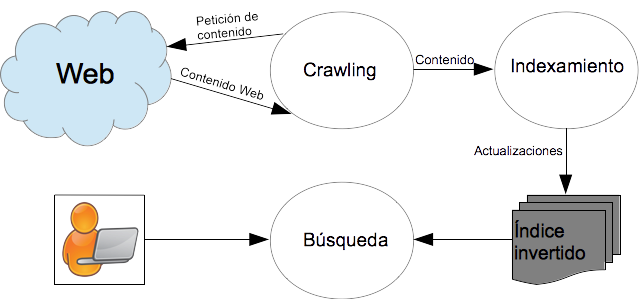
\includegraphics[scale=.75]{images/searchenginearchitecture.png}
\caption{Arquitectura típica de un motor de búsqueda}
\label{fig:searchenginearchitecture}
\end{figure}

Dado el volúmen de datos involucrado en el procesamiento, se debe tener una estructura de datos que permita encontrar cuáles páginas contienen las palabras presentes en la búsqueda, todo esto dentro de un período de tiempo aceptable. El índice invertido es una estructura de datos que contiene una lista con todas las palabras que el proceso de \textit{crawling} ha visto, y asociada a cada palabra se tiene una lista de todas las páginas Web donde ésta palabra aparece mencionada. El motor de búsqueda construye esta estructura con el objetivo de acelerar el proceso de las búsquedas que llegan al sistema. El proceso de búsqueda es el encargado de recibir la consulta, generar un \textit{ranking} de las páginas Web que contienen las palabras de la consulta y finalmente generar una respuesta. Las diversas formas de calcular la relevancia de una página Web será explicado en secciones posteriores.

En un motor de búsqueda se pueden encontrar diversos servicios tales como (a) cálculo de las mejores páginas Web para una cierta consulta; (b) construcción de la página Web con los resultados de la consulta; (c) publicidad relacionada con las \textit{queries}; (e) sugerencia de \textit{queries}; entre muchos otros servicios.

Lo que se hace hoy en día es agrupar computadores para procesar una consulta y producir la respuesta de ésta. Este conjunto de computadores recibe el nombre de \textit{cluster}.

La diferencia entre un motor de búsqueda vertical y uno general, es que el primero se centra solo en un contenido específico de la Web. El \textit{crawler} también debe extraer solo el contenido de aquellas páginas Web que están dentro del dominio permitido. Al ser un dominio acotado, las páginas Web a procesar serán menos y por tanto la lista de los términos del índice invertido serán eventualmente de menor tamaño. Sin embargo, en un motor de búsqueda vertical las actualizaciones al índice invertido ocurren con mayor frecuencia.


\section{\'Indice invertido}
\label{marco:ii}
Es una estructura de datos que contiene todos los términos (palabras) encontrados. A cada uno de los términos, está asociado una lista de punteros a los documentos (páginas Web) que contienen dicho término. Además se almacena información que permita realizar el \textit{ranking} de las respuestas a las consultas que llegan al sistema, por ejemplo, el número de veces que aparece el término en el documento. Esta lista recibe el nombre de lista invertida.

Para construir un índice invertido se debe procesar cada palabra que existe en un documento, registrando su posición y la cantidad de veces que éste se repite. Cuando se procesa el término con la información asociada correspondiente, se almacena en el índice invertido (ver Figura \ref{fig:invertedindex}).

\begin{figure}[tp]
\centering
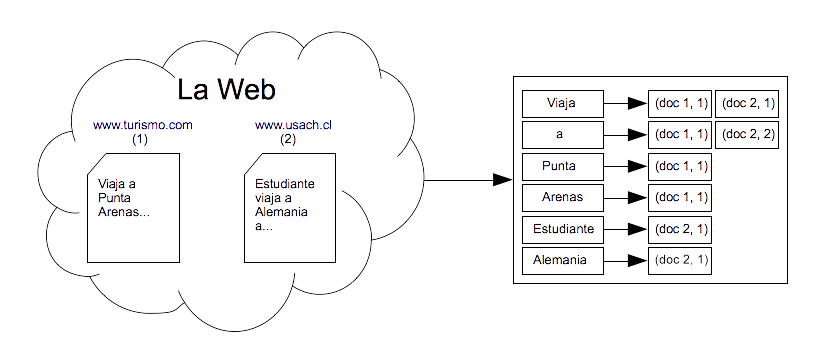
\includegraphics[scale=.75]{images/invertedindex.png}
\caption{\'Indice invertido}
\label{fig:invertedindex}
\end{figure}

El tamaño del índice invertido crece rápido y eventualmente la memoria RAM se agotará antes de procesar toda la colección de documentos. Cuando la memoria RAM se agota, se almacena en disco el índice parcial hasta aquel momento, se libera la memoria y se continúa con el proceso. Además, se debe hacer un \textit{merge} de los índices parciales uniéndo las listas invertidas de cada uno de los términos involucrados.